\chapter{User manual}\label{appendix:user_manual}

This user manual describes the steps required to build, flash, and operate the mobile robot platform. It covers firmware tooling, \gls{ros}~2 workspace setup, and operating system configuration.

\section{MCU firmware: build \& flash workflow}

\subsection{Prerequisites}
Ensure the following components are installed on Ubuntu 22.04 or equivalent:
\begin{itemize}
\item GNU Arm Embedded Toolchain v12.3-Rel1 or newer
\item CMake $\geq$ 3.25
\item OpenOCD 0.12.0 \emph{or} STM32CubeProgrammer 2.15
\item \texttt{stlink-tools} 1.7 (optional, for \texttt{st-flash})
\end{itemize}
Install via:
\begin{lstlisting}[language=bash]
sudo apt update
sudo apt install gcc-arm-none-eabi cmake make openocd stlink-tools
\end{lstlisting}

\subsection{Building the firmware}
\begin{enumerate}
\item Change into the firmware directory:
\begin{lstlisting}[language=bash]
cd MCU
\end{lstlisting}
\item Configure the build:
\begin{lstlisting}[language=bash]
cmake -B build -DCMAKE\_BUILD\_TYPE=Release
\end{lstlisting}
\item Compile:
\begin{lstlisting}[language=bash]
cmake --build build -j\$(nproc)
\end{lstlisting}
\item The outputs (\texttt{plub\_plub.elf}, \texttt{plub\_plub.bin}) will be in \texttt{MCU/build/}.
\end{enumerate}

\subsection{Flashing the firmware}
\paragraph*{Option A: OpenOCD}
\begin{lstlisting}[language=bash]
openocd -f interface/stlink.cfg
openocd -f target/stm32f4x.cfg
openocd -c "program build/plub\_plub.elf verify reset exit"
\end{lstlisting}

\paragraph*{Option B: ST-LINK CLI}
\begin{lstlisting}[language=bash]
st-flash write build/plub\_plub.bin 0x08000000
\end{lstlisting}

\noindent Verify successful programming:
\begin{lstlisting}[language=bash]
openocd -f interface/stlink.cfg
openocd -f target/stm32f4x.cfg
openocd -c "mdw 0x08000000 4"
\end{lstlisting}

\section{ROS 2 workspace setup}

\subsection{System dependencies}
Install \gls{ros}~2 Humble and related packages:
\begin{lstlisting}[language=bash]
sudo apt install ros-humble-desktop
sudo apt install python3-colcon-common-extensions
sudo apt install ros-humble-ros2-control
sudo apt install ros-humble-ros2-controllers
sudo apt install ros-humble-rosbridge-suite
sudo apt install can-utils
\end{lstlisting}

\subsection{Building the workspace}
\begin{enumerate}
\item Enter the workspace:
\begin{lstlisting}[language=bash]
cd plub\_plub\_ws
\end{lstlisting}
\item Install dependencies:
\begin{lstlisting}[language=bash]
rosdep install --from-paths src --ignore-src -y
\end{lstlisting}
\item Build:
\begin{lstlisting}[language=bash]
colcon build --symlink-install
\end{lstlisting}
\item Source:
\begin{lstlisting}[language=bash]
source ./install/setup.bash
\end{lstlisting}
\end{enumerate}

\subsection{Launching the full stack}
\begin{lstlisting}[language=bash]
ros2 launch run run.launch.py
\end{lstlisting}

\section{Operating system configuration}

\subsection{Serial \& USB permissions}
Grant access to the USB serial port:
\begin{lstlisting}[language=bash]
sudo chmod 777 /dev/ttyUSB0
lsusb \
  | awk '/03e7/ { gsub(/:$/,"",$4); printf "/dev/bus/usb/%03d/%03d\n", $2, $4 }' \
  | xargs sudo chmod 666
\end{lstlisting}

\subsection{CAN channel initialization}
\begin{lstlisting}[language=bash]
sudo ip link set can1 type can bitrate 500000
sudo ip link set can1 up
candump can1
\end{lstlisting}

\chapter{Comprehensive parameter listing}\label{app:launch_params}

To ensure full experimental reproducibility, this appendix exhaustively
enumerates the runtime parameters that are injected into each \gls{ros}~2 node at
launch. Unless otherwise stated, the values correspond to those employed
throughout the evaluation campaign presented in Chapter~\ref{ch:implementation}. Boolean parameters are listed as \texttt{true}/\texttt{false};
hexadecimal integers are formatted with a \texttt{0x}~prefix.

%-------------------------------------------------------------------------------
\section{\texttt{can\_communication} package}
\subsection{\texttt{can\_node}}
\begin{longtable}{@{}llp{0.60\textwidth}@{}}
  \toprule
  \textbf{Parameter} & \textbf{Type} & \textbf{Description} \\
  \midrule
  \endhead
  can\_interface      & string & Host \gls{can} interface bound to the socket. \\[-4pt]
  tx\_can\_id          & uint32 & Arbitration ID used for outgoing frames. \\[-4pt]
  rx\_can\_id          & uint32 & Hardware filter mask for incoming frames. \\[-4pt]
  bitrate             & uint32 & Bus bitrate in \nicefrac{bits}{sec}. \\[-4pt]
  filter\_incoming     & bool   & Enables kernel level RX filtering. \\
  \bottomrule
\end{longtable}

\section{\texttt{ldlidar\_ros2} package}
\subsection{\texttt{ldlidar\_ros2\_node}}
\begin{longtable}{@{}llp{0.60\textwidth}@{}}
  \toprule
  \textbf{Parameter} & \textbf{Type} & \textbf{Description} \\
  \midrule
  product\_name            & string & LiDAR model identifier. \\[-4pt]
  topic\_name              & string & Topic onto which the \texttt{sensor\_msgs/LaserScan} is published. \\[-4pt]
  frame\_id                & string & Reference frame attached to the LiDAR optical centre. \\[-4pt]
  port\_name               & string & Serial device path of the bridge. \\[-4pt]
  laser\_scan\_dir         & bool   & \texttt{true}: counter/clockwise; \texttt{false}: clockwise scan order. \\[-4pt]
  enable\_angle\_crop\_func & bool   & Activates angular masking of the raw scan. \\[-4pt]
  angle\_crop\_min         & float  & Inclusive lower bound of the angular mask (\si{\degree}). \\[-4pt]
  angle\_crop\_max         & float  & Inclusive upper bound of the angular mask (\si{\degree}). \\
  \bottomrule
\end{longtable}

\section{\texttt{mecanum\_drive} package}\label{app:mecanum_drive_params}

\subsection{\texttt{mecanum\_drive\_controller}}

\begin{longtable}{@{}lll@{}}
\toprule
\textbf{Parameter} & \textbf{Value} & \textbf{Description} \\
\midrule
ticks\_per\_meter          & 4332.0 & Encoder ticks that correspond to one metre of tangential wheel travel. \\
wheel\_separation          & 0.34   & Lateral distance between the mid points of the left and right wheel contact patches (m). \\
wheel\_separation\_length  & 0.24   & Longitudinal distance between the front and rear axle lines (m). \\
max\_motor\_speed          & 3456   & Upper bound on the actuator command (\nicefrac{ticks}{second}). \\
\bottomrule
\end{longtable}

\subsection{\texttt{mecanum\_drive\_odometry}}

\begin{longtable}{@{}lll@{}}
\toprule
\textbf{Parameter} & \textbf{Value} & \textbf{Description} \\
\midrule
ticks\_per\_meter          & 4332.0 & Same conversion factor as for the controller, ensuring kinematic coherence. \\
wheel\_separation          & 0.34   & Lateral baseline (m). \\
wheel\_separation\_length  & 0.24   & Longitudinal baseline (m). \\
base\_frame\_id            & \texttt{base\_link} & Name of the robot's body frame in the \textsf{tf2} tree. \\
odom\_frame\_id            & \texttt{odom}       & Fixed world frame used for integrating wheel displacements. \\
encoder\_min               & $-32\,768$ & Lower bound of the 16-bit encoder counter. \\
encoder\_max               & $32\,767$  & Upper bound of the 16-bit encoder counter. \\
\bottomrule
\end{longtable}

\section{\texttt{depthai\_ros\_driver} package}
The OAK-D camera driver is launched via the vendor/supplied
\texttt{camera.launch.py}. The only top/level parameters injected by
\texttt{global.launch.py} are the camera namespace (name) and the
path to an external YAML file (params\_file). The contents of that
YAML are vendor maintained and excluded here for brevity.

\section{\texttt{rtabmap\_slam} package}

\begin{longtable}{@{}llp{0.60\textwidth}@{}}
  \toprule
  \textbf{Parameter} & \textbf{Value} & \textbf{Description} \\
  \midrule
  \endhead
  frame\_id                      & \texttt{base\_link}  & align data with the vehicle frame. \\[-4pt]
  subscribe\_rgb                 & \texttt{true}        & enable RGB stream subscription. \\[-4pt]
  subscribe\_depth               & \texttt{true}        & enable aligned depth stream subscription. \\[-4pt]
  subscribe\_scan                & \texttt{true}        & fuse 2D LiDAR scan into occupancy grid. \\[-4pt]
  subscribe\_odom\_info          & \texttt{false}       & disable odometry info subscription. \\[-4pt]
  subscribe\_imu                 & \texttt{false}       & disable IMU data subscription. \\[-4pt]
  sync\_queue\_size              & \texttt{10}          & bound message filter queue length. \\[-4pt]
  approx\_sync                   & \texttt{true}        & enforce approximate time synchronization heuristic. \\[-4pt]
  approx\_sync\_max\_interval    & \SI{0.001}{s}        & maximum allowed timestamp difference for sync. \\[-4pt]
  visual\_odometry               & \texttt{false}       & disable visual odometry feature. \\[-4pt]
  delete\_db\_on\_start          & \texttt{true}        & clear the database at startup. \\[-4pt]
  FAST/gpu                       & \texttt{true}        & enable GPU acceleration for FAST feature detection. \\[-4pt]
  Grid/Sensor                    & \texttt{0}           & sensor ID to use for occupancy grid integration (LiDAR). \\[-4pt]
  RGBD/NeighborLinkRefining      & \texttt{true}        & refine graph links between spatially close nodes. \\[-4pt]
  RGBD/ProximityBySpace          & \texttt{true}        & create links based on spatial proximity. \\[-4pt]
  RGBD/AngularUpdate             & \num{0.05}           & angular threshold (rad) for creating a new keyframe. \\[-4pt]
  RGBD/LinearUpdate              & \num{0.05}           & linear threshold (m) for creating a new keyframe. \\[-4pt]
  Grid/RangeMax                  & \SI{11.5}{m}         & clip occupancy grid integration beyond this radius. \\[-4pt]
  Grid/RangeMin                  & \SI{0.5}{m}          & ignore depth measurements closer than this radius. \\[-4pt]
  Grid/FromDepth                 & \texttt{false}       & disable building grid directly from depth images. \\[-4pt]
  Reg/Force3DoF                  & \texttt{true}        & constrain on odometry ($x,y,\theta$). \\[-4pt]
  Reg/Strategy                   & \texttt{1}           & registration strategy selector. \\[-4pt]
  RGBD/ProximityByTime           & \texttt{false}       & disable linking based on temporal proximity. \\[-4pt]
  RGBD/ProximityPathMaxNeighbors & \texttt{10}          & max neighbors to consider in proximity path search. \\[-4pt]
  RGBD/LocalRadius               & \num{5}              & radius (m) for local link detection. \\[-4pt]
  Vis/MinInliers                 & \texttt{10}          & minimum inliers required for visual registration. \\[-4pt]
  RGBD/OptimizeFromGraphEnd      & \texttt{false}       & disable incremental optimization from graph end. \\[-4pt]
  RGBD/OptimizeMaxError          & \texttt{4}           & maximum allowed error for graph optimization. \\[-4pt]
  Icp/CorrespondenceRatio        & \num{0.2}            & ratio of correspondences to keep during ICP. \\[-4pt]
  Icp/PM                         & \texttt{false}       & disable point-to-mesh correspondence. \\[-4pt]
  Icp/PointToPlane               & \texttt{false}       & disable point-to-plane ICP mode. \\[-4pt]
  Icp/MaxCorrespondenceDistance  & \SI{0.1}{m}          & tighter point-plane ICP constraint. \\[-4pt]
  Icp/VoxelSize                  & \SI{0.05}{m}         & down/up-sample point clouds for ICP. \\
  \bottomrule
\end{longtable}


The remaining parameters retain their package
defaults and are therefore omitted.

\chapter{extended results}\label{app:extended_results}

This appendix provides additional results that were not included in the main body of the thesis. The data presented here is intended to support the findings and conclusions drawn in the results chapter.
A photo of the 3D reconstructions and scene from robot perspective is shown in each figure.

\begin{figure}[H]
  \centering
  \begin{subfigure}[b]{0.47\textwidth}
    \centering
    \includegraphics[height=6cm,width=\textwidth]{imgs/lc1.png}
    \caption{Point cloud}

  \end{subfigure}
  \hfill
  \begin{subfigure}[b]{0.47\textwidth}
    \centering
    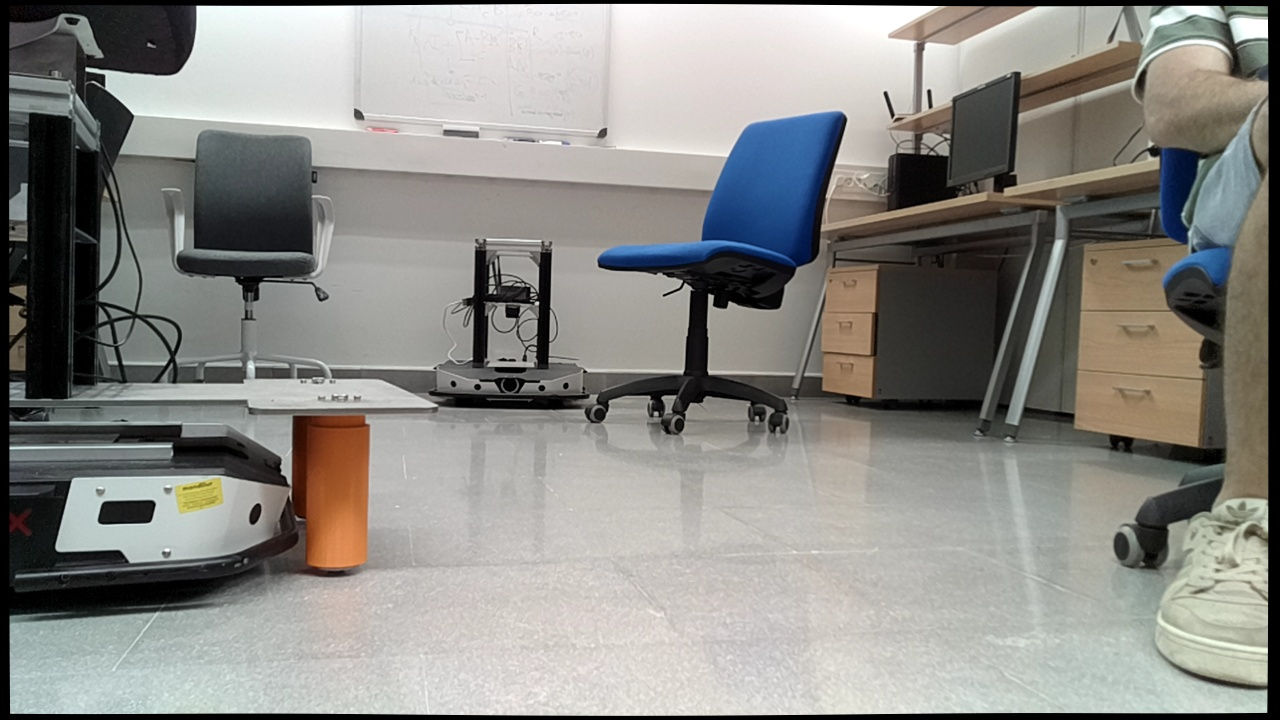
\includegraphics[height=6cm,width=\textwidth]{imgs/lr1.png}
    \caption{RGB}

  \end{subfigure}
\end{figure}

\begin{figure}[H]
  \centering
  \begin{subfigure}[b]{0.47\textwidth}
    \centering
    \includegraphics[height=6cm,width=\textwidth]{imgs/lc3.png}
    \caption{Point cloud}

  \end{subfigure}
  \hfill
  \begin{subfigure}[b]{0.47\textwidth}
    \centering
    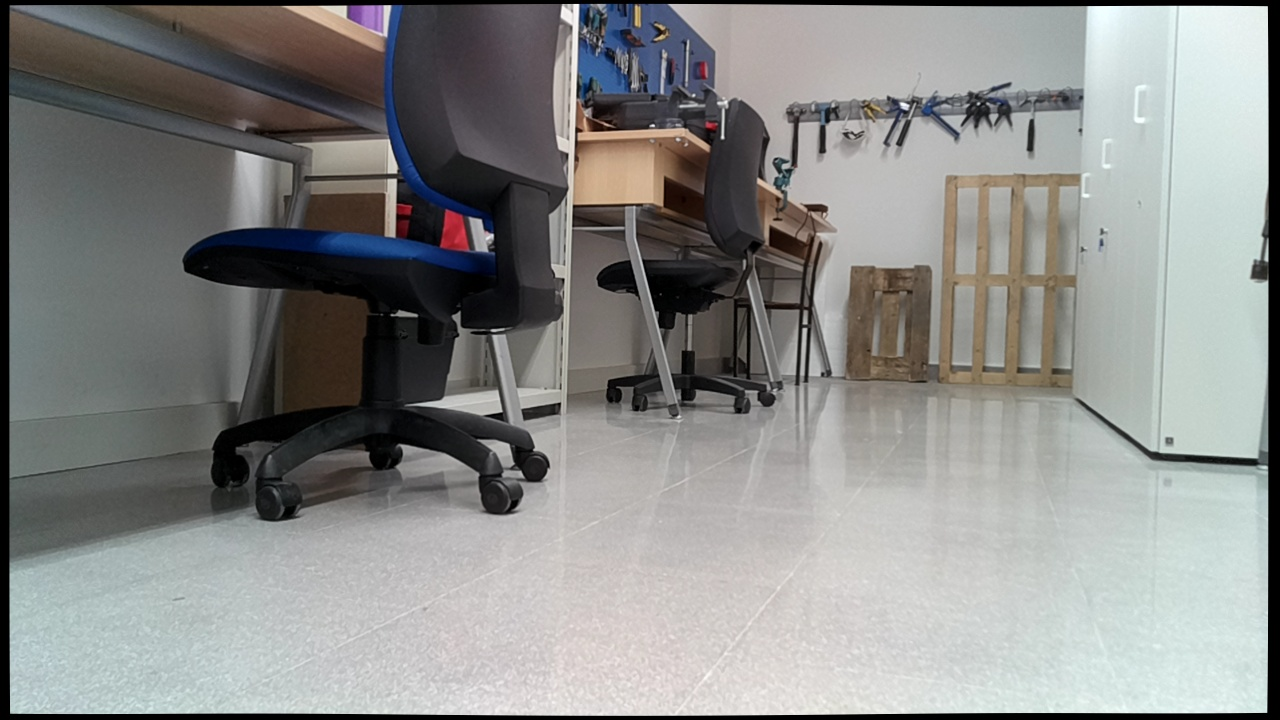
\includegraphics[height=6cm,width=\textwidth]{imgs/lr3.png}
    \caption{RGB}

  \end{subfigure}
\end{figure}

\begin{figure}[H]
  \centering
  \begin{subfigure}[b]{0.47\textwidth}
    \centering
    \includegraphics[height=6cm,width=\textwidth]{imgs/lc4.png}
    \caption{Point cloud}

  \end{subfigure}
  \hfill
  \begin{subfigure}[b]{0.47\textwidth}
    \centering
    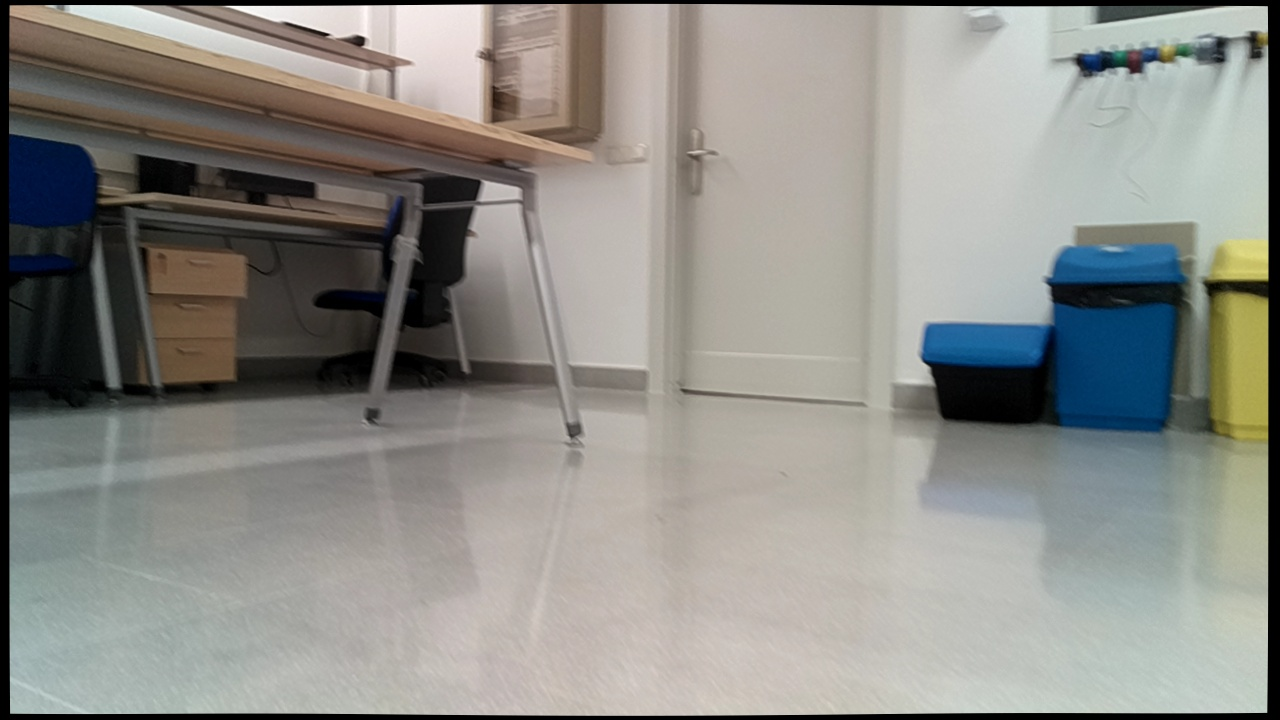
\includegraphics[height=6cm,width=\textwidth]{imgs/lr4.png}
    \caption{RGB}

  \end{subfigure}
\end{figure}

\begin{figure}[H]
  \centering
  \begin{subfigure}[b]{0.47\textwidth}
    \centering
    \includegraphics[height=6cm,width=\textwidth]{imgs/lc5.png}
    \caption{Point cloud}

  \end{subfigure}
  \hfill
  \begin{subfigure}[b]{0.47\textwidth}
    \centering
    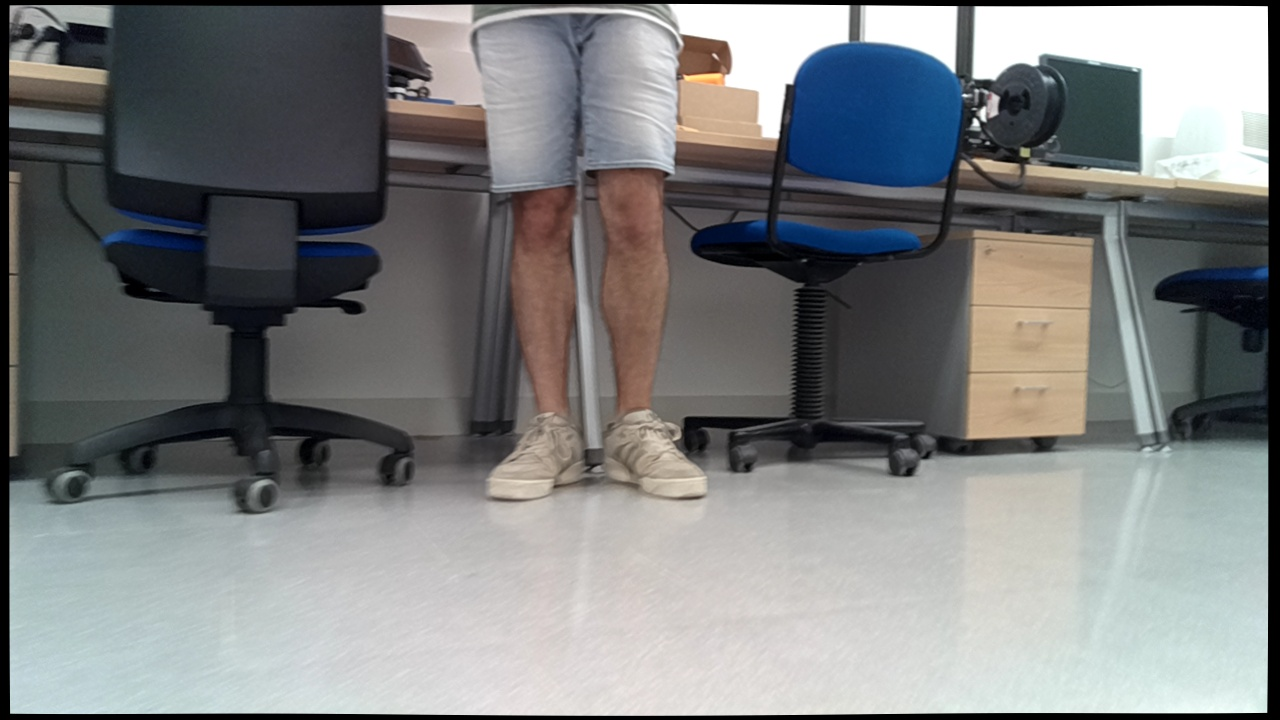
\includegraphics[height=6cm,width=\textwidth]{imgs/lr5.png}
    \caption{RGB}

  \end{subfigure}
\end{figure}

\begin{figure}[H]
  \centering
  \begin{subfigure}[b]{0.47\textwidth}
    \centering
    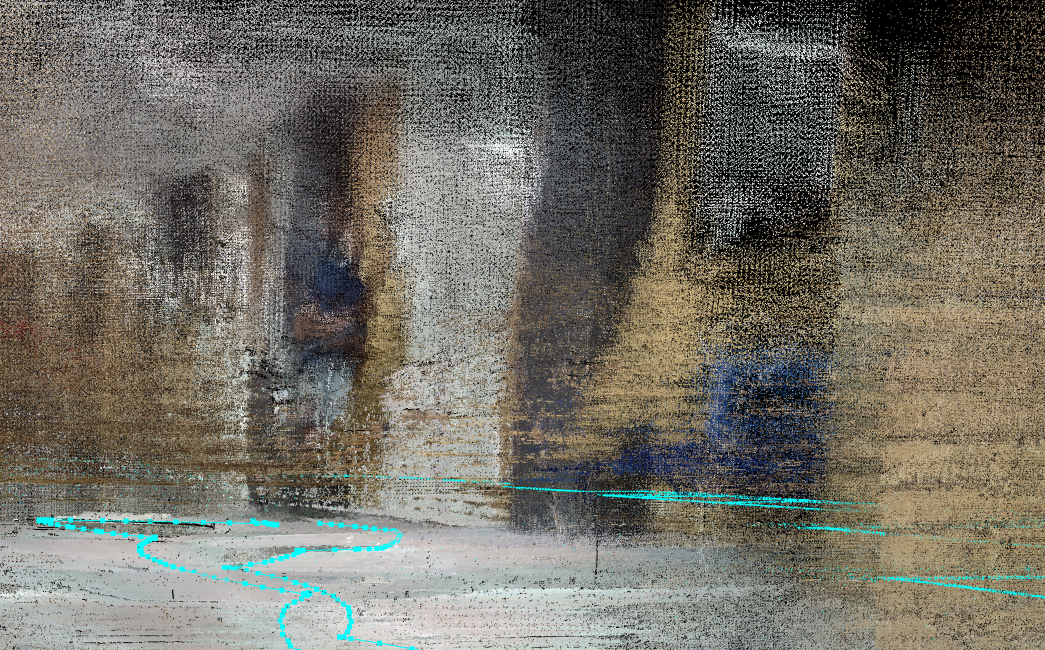
\includegraphics[height=6cm,width=\textwidth]{imgs/cc (1).png}
    \caption{Point cloud}

  \end{subfigure}
  \hfill
  \begin{subfigure}[b]{0.47\textwidth}
    \centering
    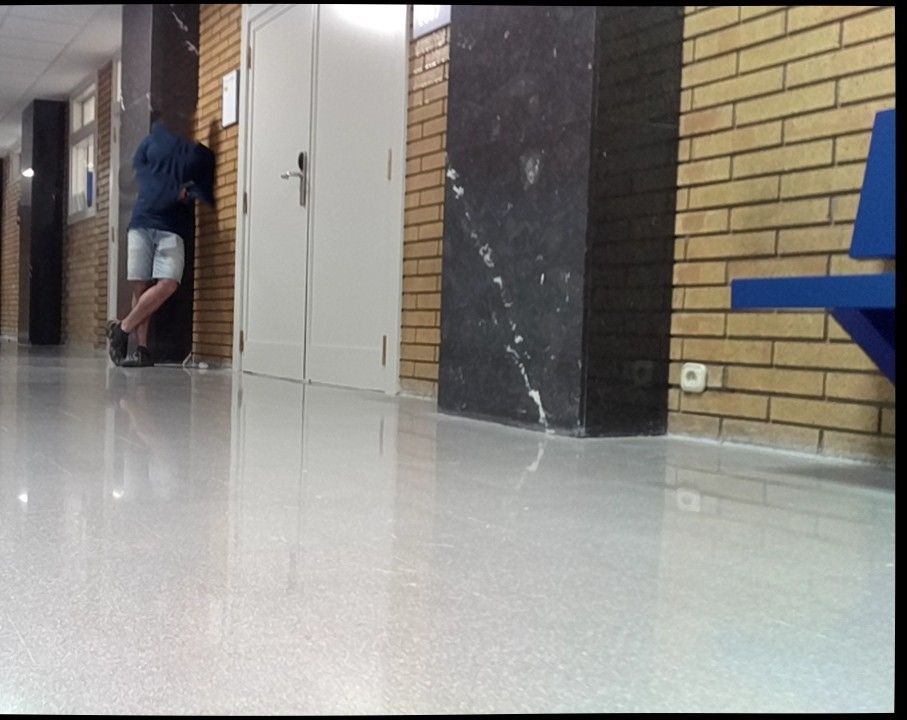
\includegraphics[height=6cm,width=\textwidth]{imgs/cr1.jpg}
    \caption{RGB}

  \end{subfigure}
\end{figure}

\begin{figure}[H]
  \centering
  \begin{subfigure}[b]{0.47\textwidth}
    \centering
    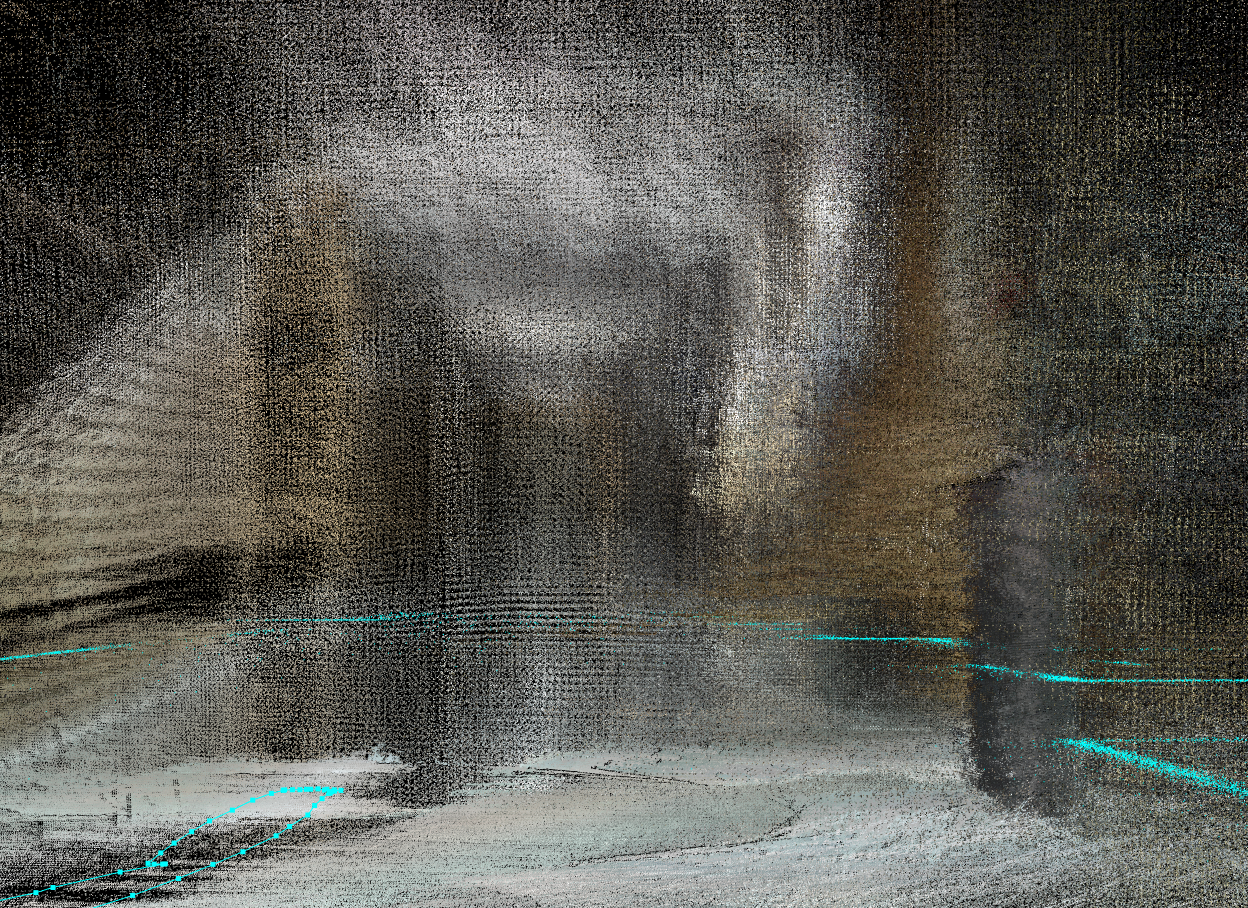
\includegraphics[height=6cm,width=\textwidth]{imgs/cc (4).png}
    \caption{Point cloud}

  \end{subfigure}
  \hfill
  \begin{subfigure}[b]{0.47\textwidth}
    \centering
    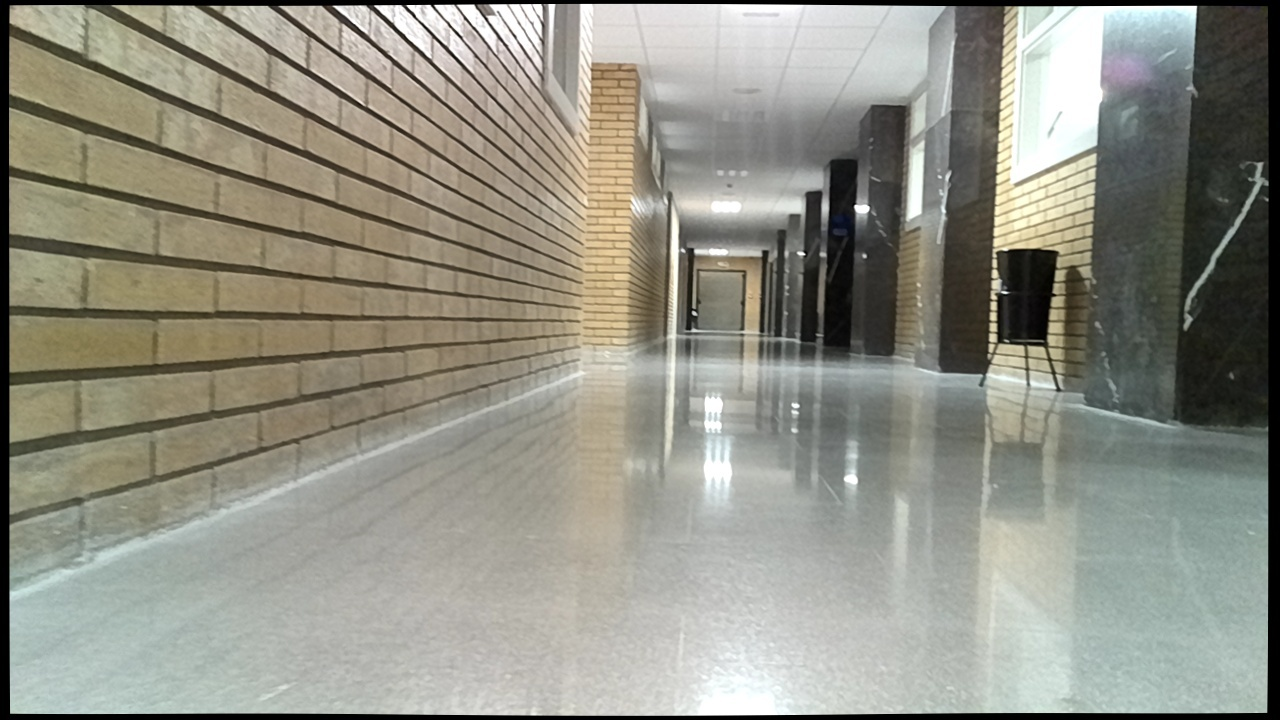
\includegraphics[height=6cm,width=\textwidth]{imgs/cr4.jpg}
    \caption{RGB}

  \end{subfigure}
\end{figure}

\begin{figure}[H]
  \centering
  \begin{subfigure}[b]{0.47\textwidth}
    \centering
    \includegraphics[height=6cm,width=\textwidth]{imgs/cc (3).png}
    \caption{Point cloud}

  \end{subfigure}
  \hfill
  \begin{subfigure}[b]{0.47\textwidth}
    \centering
    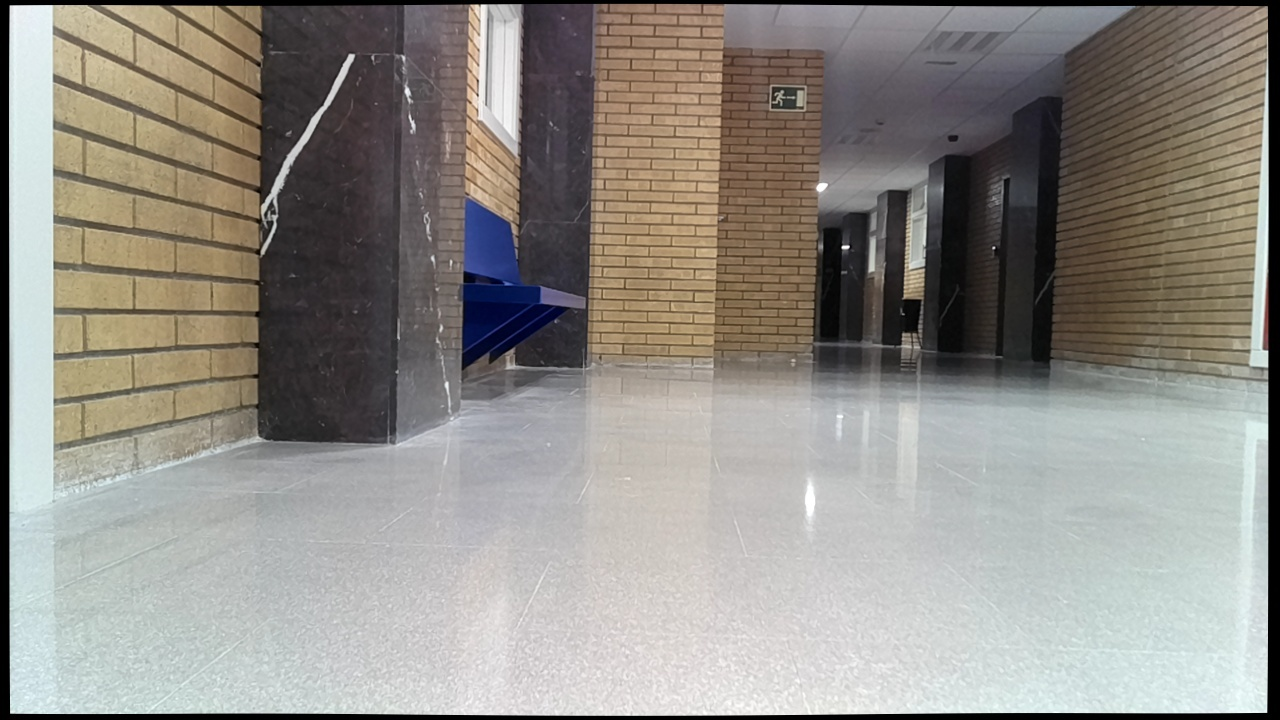
\includegraphics[height=6cm,width=\textwidth]{imgs/cr3.jpg}
    \caption{RGB}

  \end{subfigure}
\end{figure}